\section{Cohorts matter: Variation in activity, effort, survival}

\subsection{Users' Activity}

One common metric of interest of a social network is the average number of posts that active users make in a determined time frame. For reddit, in particular, the overall evolution of monthly average posts per user is as follows.

\begin{figure}[!tb]
\centering
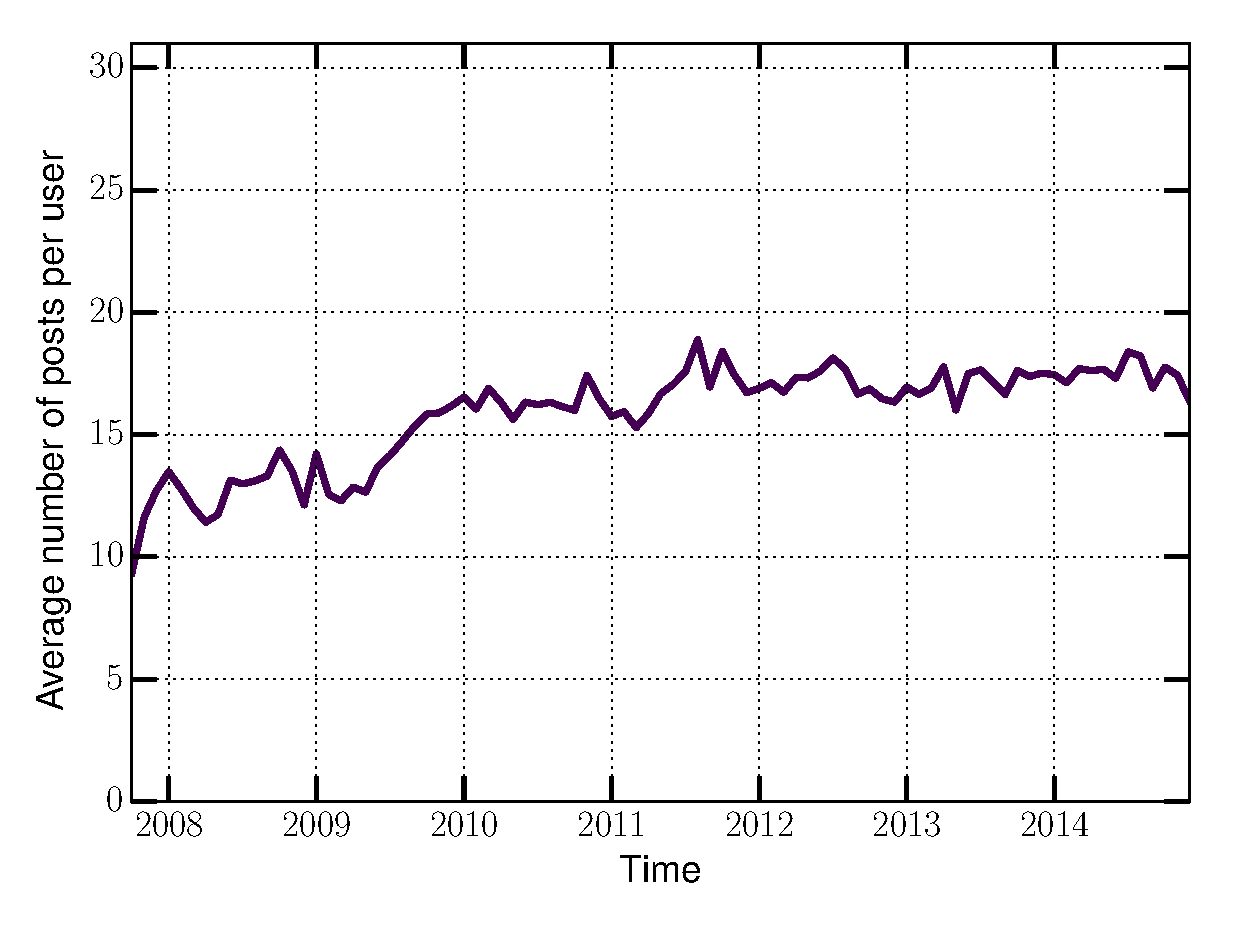
\includegraphics[scale=0.4]{./images/avr_posts_per_user_over_time_total.eps}
\caption{Caption}
\label{fig:avr_posts_per_user_over_time_total}
\end{figure}

This is the first and most naive approach one can make to analyze the evolution of posting behavior for the users. This figure, however, averages over all active users in each evaluated time step. This hides cohort effects due to the user behavior evolution over the years of existence of the network. A first attempt to improve this would be to evaluate this posting average according to the users cohorts, as shown in Figure N.

\begin{figure}[!tb]
\centering
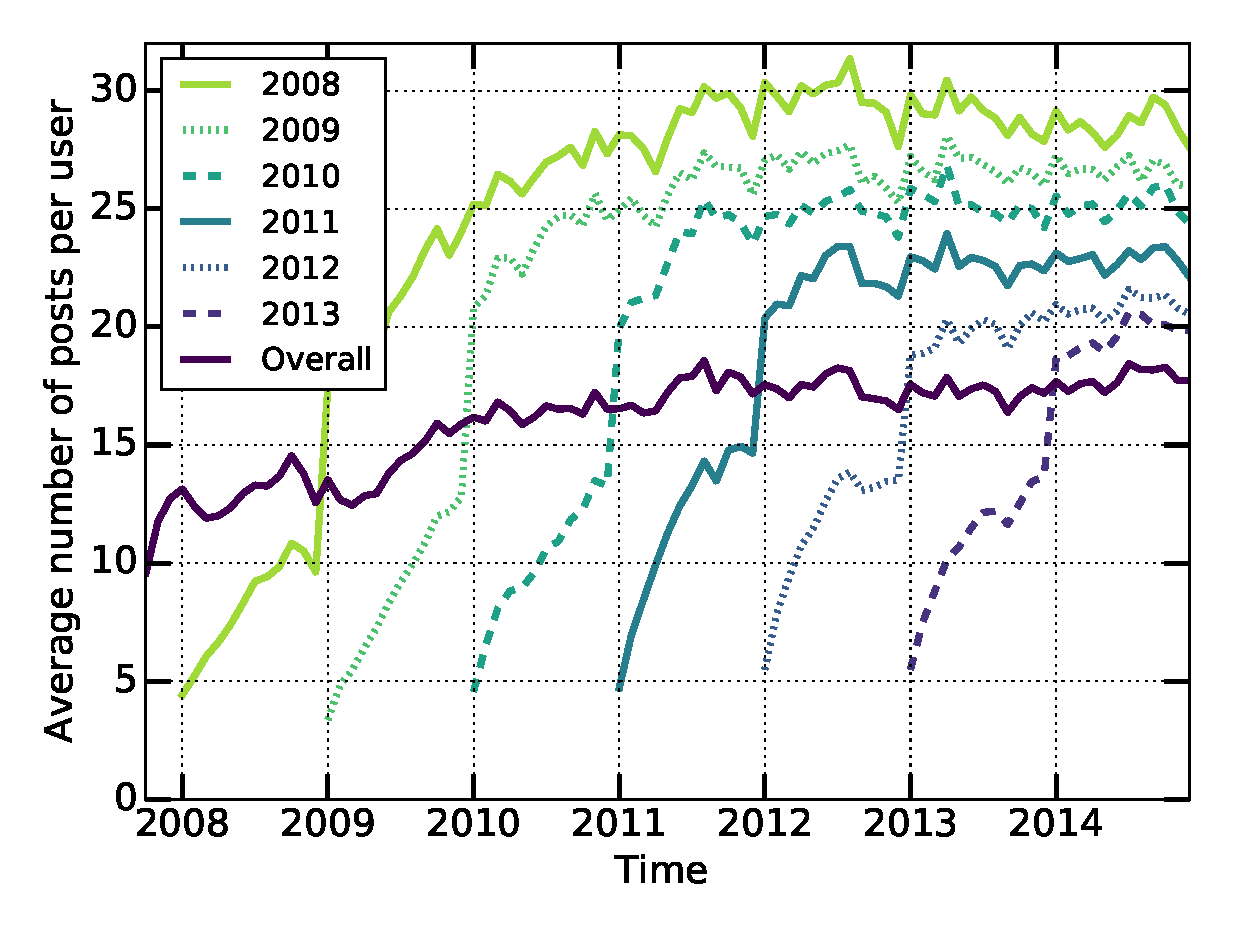
\includegraphics[scale=0.4]{./images/avr_posts_per_user_over_time_cohorts.eps}
\caption{Caption}
\label{fig:avr_posts_per_user_over_time_cohorts}
\end{figure}

Here we notice already a significant cohort effect: users from latter cohorts have a significantly lower posting average than users from earlier cohorts.

There are, however, two possible pitfalls in this analysis. The first is the fact that we are always considering the surviving users, that is, we count the users that presented some activity on the said month. Based on this, users from older cohorts could be posting more on average in 2014 because they are the ones that survived the longest and possibly are the ones that are most interested and get the most value out of the network, which would justify the increasing activity over.

To account for this, we change our time referential: each post time is considered as the time since the user creation (in our analysis, this referential is the first observed post for the user). This allows us to compare users based on how long they have existed in the network (but still treat them as cohorts), as seen in Figure N.

The second pitfall that one should be careful with is that users are being created during the cohort year, but not anymore afterwards. This accounts for the sharp increase in the average number of posts in Figure N. Since we segmented our users by cohorts, by the end of each year onwards, we do not have users joining the network anymore and the number of active users does not increase because of new users anymore. This fact, associated with the fact that young users tend to post less, drag the average down during the year, since young users are always coming in the network. This effect is more clear in Figure N, when we use the user-referential time frame, where it is clear that young users post less. This is particularly true for the first month, specially considering that there are many user accounts that are created and only show activity for a single day in reddit, which likely brings the average down.

\begin{figure}[!tb]
\centering
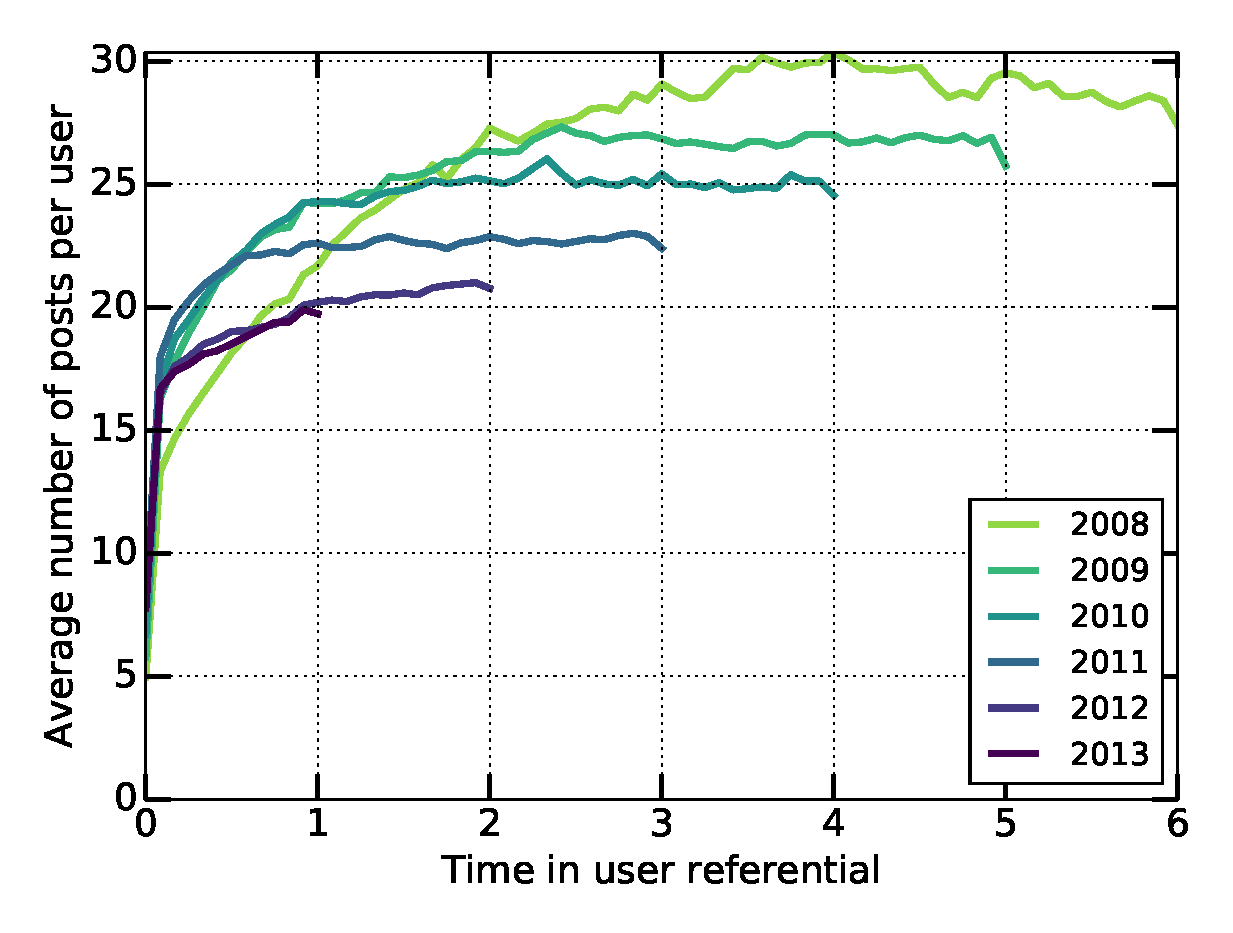
\includegraphics[scale=0.4]{./images/avr_posts_per_user_cohorts.eps}
\caption{Caption}
\label{fig:avr_posts_per_user_cohorts}
\end{figure}

It is unclear if in the initial year of existence of the users there are significant cohort effects in the average number of posts. However, we can observe that different cohorts apparently stabilize in different levels of behavior, with a general tendency for older cohorts leveling at lower values, eg. people from 2008 and 2009 level at higher posting frequencies than 2010. Some possible explanations for this would be that users that get most of the utility from the network are more likely to find it earlier, and this accounts for the higher activity for earlier cohorts. Also, earlier users could hold more status in the network, since they joined in an earlier stage of the network and therefore present a higher activity. Yet another explanation would be that earlier users demographics were different in terms of age and interests, for example, and these correlate to the fact that they present a higher activity.

\subsection{Users' Effort}

In addition to the raw number of posts, comments length can also be considered as a proxy for user effort in the network. Users that type more put more of their time in the network, contribute with more content and might create stronger ties with the community. The Figure N shows the evolution of the monthly average comment length in reddit.

\begin{figure}[!tb]
\centering
\includegraphics[scale=0.4]{./images/avr_comment_size_over_time_total.eps}
\caption{Caption}
\label{fig:avr_comment_size_over_time_total}
\end{figure}

Based on the downwards tendency of the comment length, one could possibly imagine that the user commitment with the network is lowering over time. This, however, might not be the best way to interpret this information. Figure N shows the comment length per cohort based on the user referential time. This figure shows that, unlike the average overall network comment length, surviving users increase the size of their contributions to the community over time. This is true for all users cohorts. The important thing to notice here is that, while user comments get longer as they stay for longer in the network, younger users start from a lower baseline comment than older users. Together with the fact that recent reddit has experienced exponential-like growth, the heavier weight when evaluating the averages for Figure N as the years go by is shifted towards the size of the ever growing younger generation, and this younger generation brings the average down since they start writing less.

Some possible explanations for this difference in the starting points could be that older users are, again, sampled from a different demographics that is more committed and willing to spend more effort into developing their virtual identity. Also, it could be that it is a natural evolution of the community, as older users have taken most of the main space of interests when it comes to creating new subreddits and starting these communities, new users have it all already made and sometimes might feel intimidated or not motivated to create new topics or communities that already exist or that are less likely to compete with the existing ones. In a way, these new users could behave more as lurkers, while the older users are the ones that laid the foundation of reddit.

\begin{figure}[!tb]
\centering
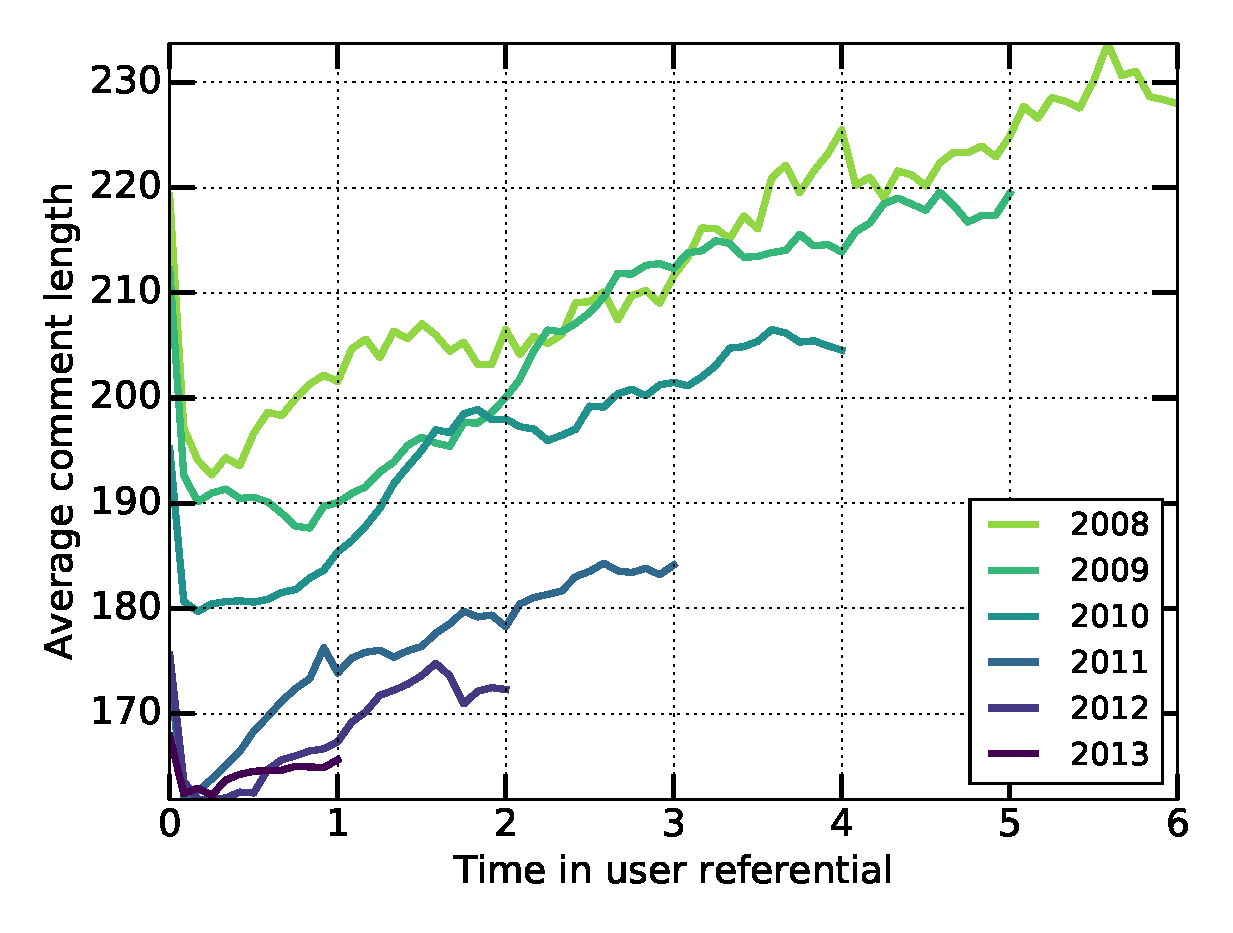
\includegraphics[scale=0.4]{./images/avr_comment_size_cohorts.eps}
\caption{Caption}
\label{fig:fig_label}
\end{figure}

Yet another hypothesis that we might consider is that users are lowering their activity due to an ``initial value problem''. We can imagine that users, as they join the network, they tend to produce content according to the norms of what they see. If we look at the cohort posting size over time superimposed with the average size for the whole network, we can see that the starting point of each cohort seems to agree to a reasonable extent to the average over the total network. This way, users would be simply reproducing things as they see in their early months, but as we have seen in Figure N, users start their life posting longer content, but there is a strong decrease in size for the early months before the size increases for the surviving users.

\begin{figure}[!tb]
\centering
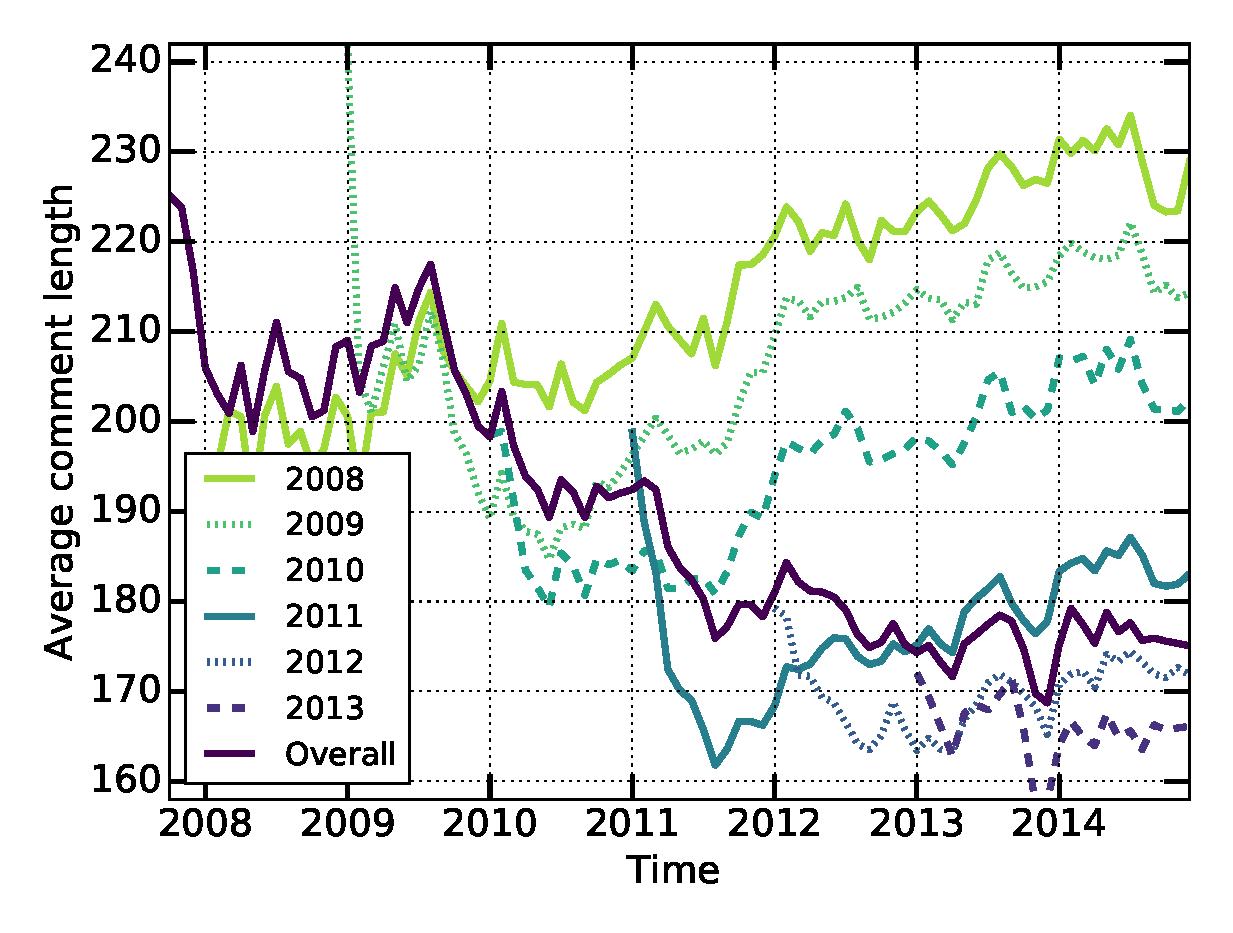
\includegraphics[scale=0.4]{./images/avr_comment_size_over_time_cohorts.eps}
\caption{Caption}
\label{fig:fig_label}
\end{figure}

\subsection{Activity Nature}

One common question from the literature is what sorts of activities users engage in; this can be used as a metric of community health (cites) or to categorize users into roles they play in the community (cite).  In reddit, we do not have per-user voting behavior, but we do have the number of comments and submissions, and a naive view of this would look at the ratio of comments to submissions over time.

While submissions can be considered new content that an author generates, a comment can be considered as a contribution to an existing content from another author. Since the total number of comments always surpasses the number of submissions, Figure N shows the evolution of the ratio of comments per submission over time for users created from 2008 until 2013. It is important to highlight here that we are not talking about the average number of comments a submission gets, but how many comments a user authors for each of his/her submissions.

\begin{figure}[!tb]
\centering
\includegraphics[scale=0.4]{./images/comments_per_submissions_over_time_total.eps}
\caption{Caption}
\label{fig:comments_per_submissions_over_time_total}
\end{figure}

We have found that segmenting users and subreddits by cohorts on the years that of the first comment highlights significant differences of behavior and help us to understand how reddit changed over these years.


Table 1: Number of distinct users that authored comments and submissions segmented by the year of the first post of the user. The Total numbers are based on posting data from 2007 until 2014, corresponding to our full dataset. The Oct 1st, 2014 onwards numbers are based on the last 3 months of data we have, and we consider this as the current, active reddit.


Table 2: Number of distinct subreddits segmented by the year of the first post of the user. The Total numbers are based on posting data from 2007 until 2014, corresponding to our full dataset. The Oct 1st, 2014 onwards numbers are based on the last 3 months of data we have, and we consider this as the current, active reddit.

Table indicates that reddit grew significantly from 2007 until 2012, practically doubling the number of new users per year for each of these years, with similarly significant growth in subreddits. Although the most expansive growth happened in the first years, more than half of the registered users are from the last 2 years, and their behavior is significantly different than previous users, impacting in the overall behavior of the community. For instance, users from the 2014 cohort have a higher tendency to make submissions instead of comments, in contrast with all the previous cohorts.

Looking at the user time referential, the evolution of the number of comments per submission shows a decreasing trend for the older cohorts. One explanation for this is that, as the community grew, more content from an absolute point of view was present in the social network, and therefore users had more reason to make contributions commenting instead of submitting new content that was likely to already exist.

\begin{figure}[!tb]
\centering
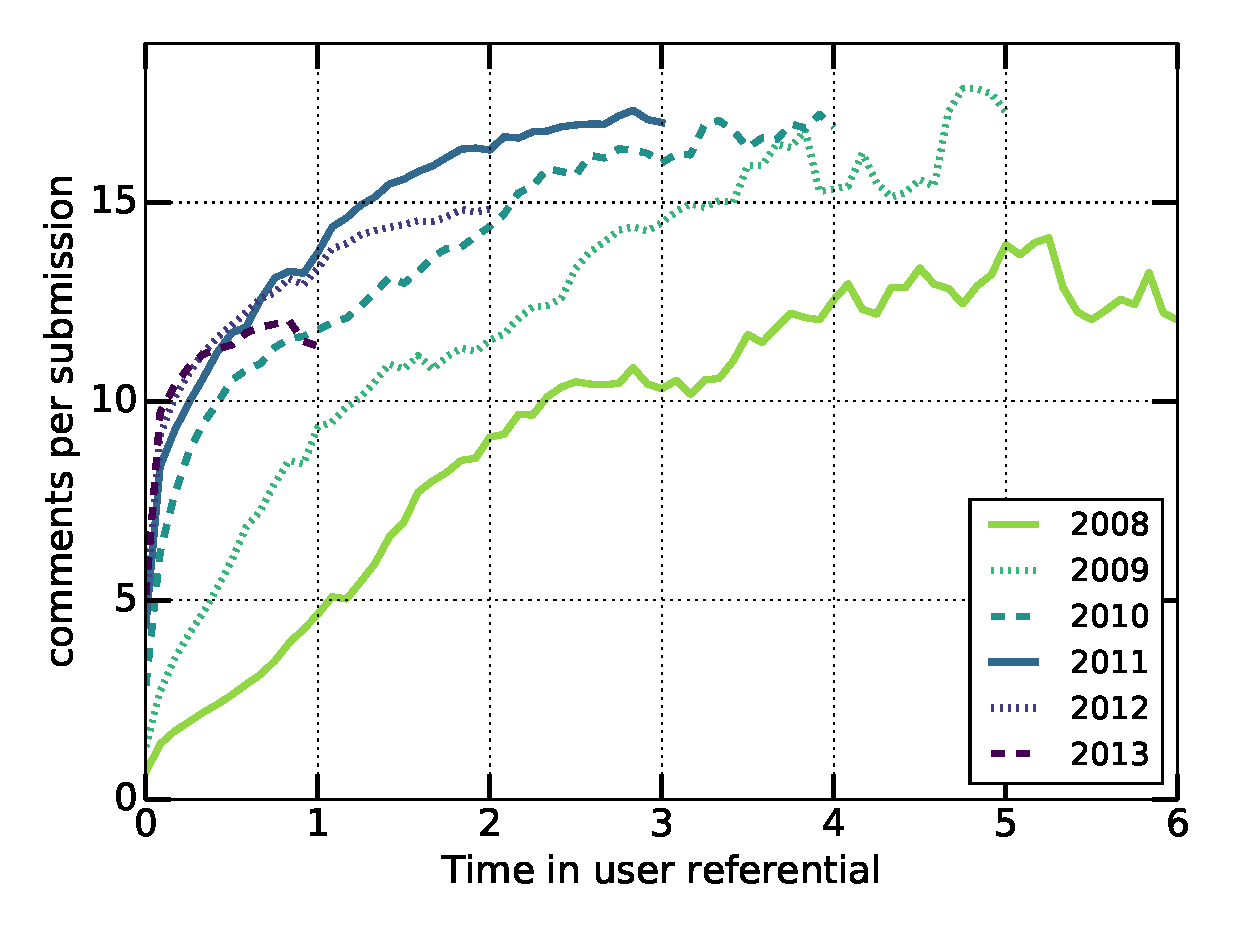
\includegraphics[scale=0.4]{./images/comments_per_submissions_cohorts.eps}
\caption{Caption}
\label{fig:comments_per_submissions_cohorts}
\end{figure}

\begin{figure}[!tb]
\centering
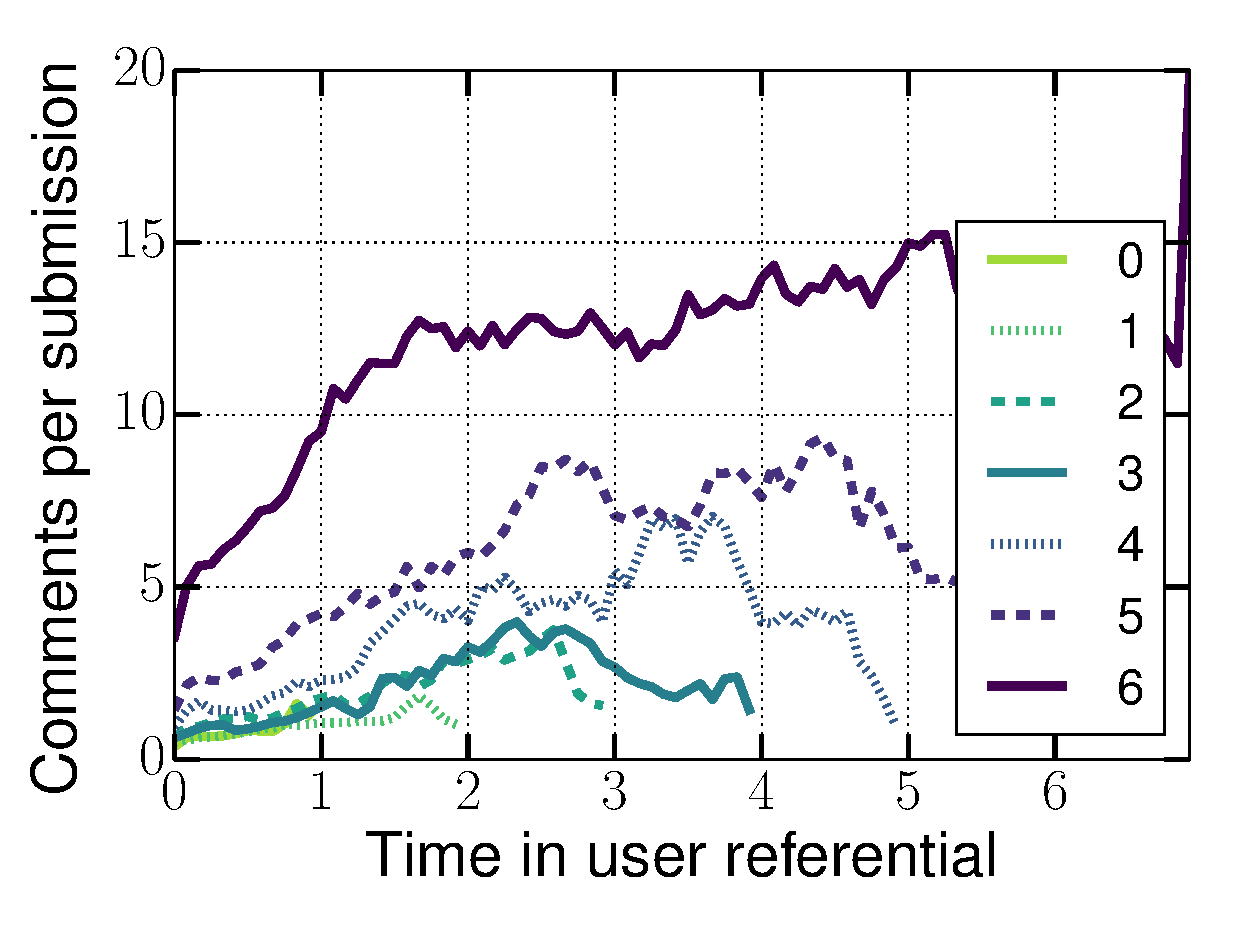
\includegraphics[scale=0.4]{./images/comments_per_submissions_for_surviving_year_for_2008.eps}
\caption{Caption}
\label{fig:comments_per_submissions_for_surviving_year_for_2008}
\end{figure}

\begin{figure}[!tb]
\centering
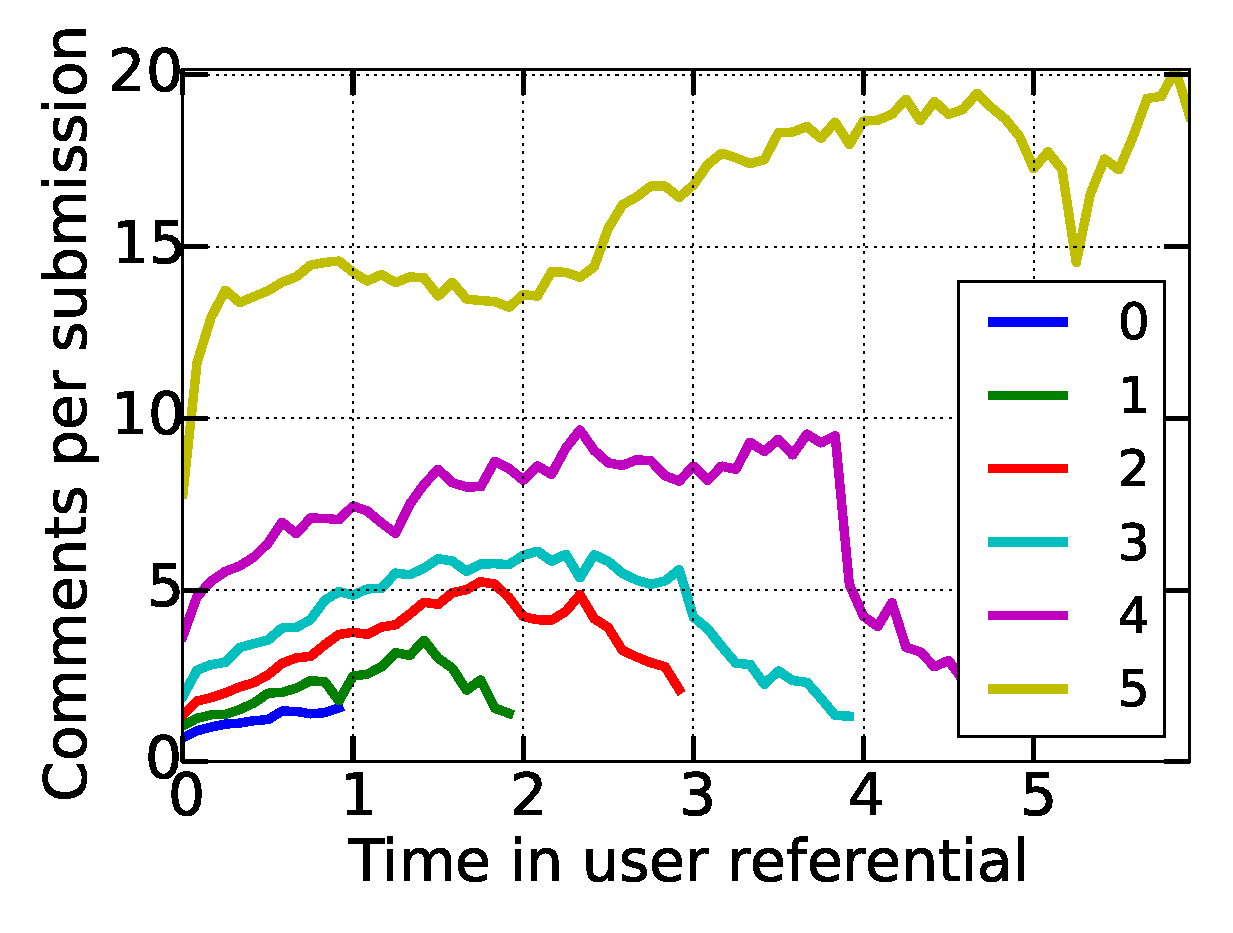
\includegraphics[scale=0.4]{./images/comments_per_submissions_for_surviving_year_for_2009.eps}
\caption{Caption}
\label{fig:comments_per_submissions_for_surviving_year_for_2009}
\end{figure}

\begin{figure}[!tb]
\centering
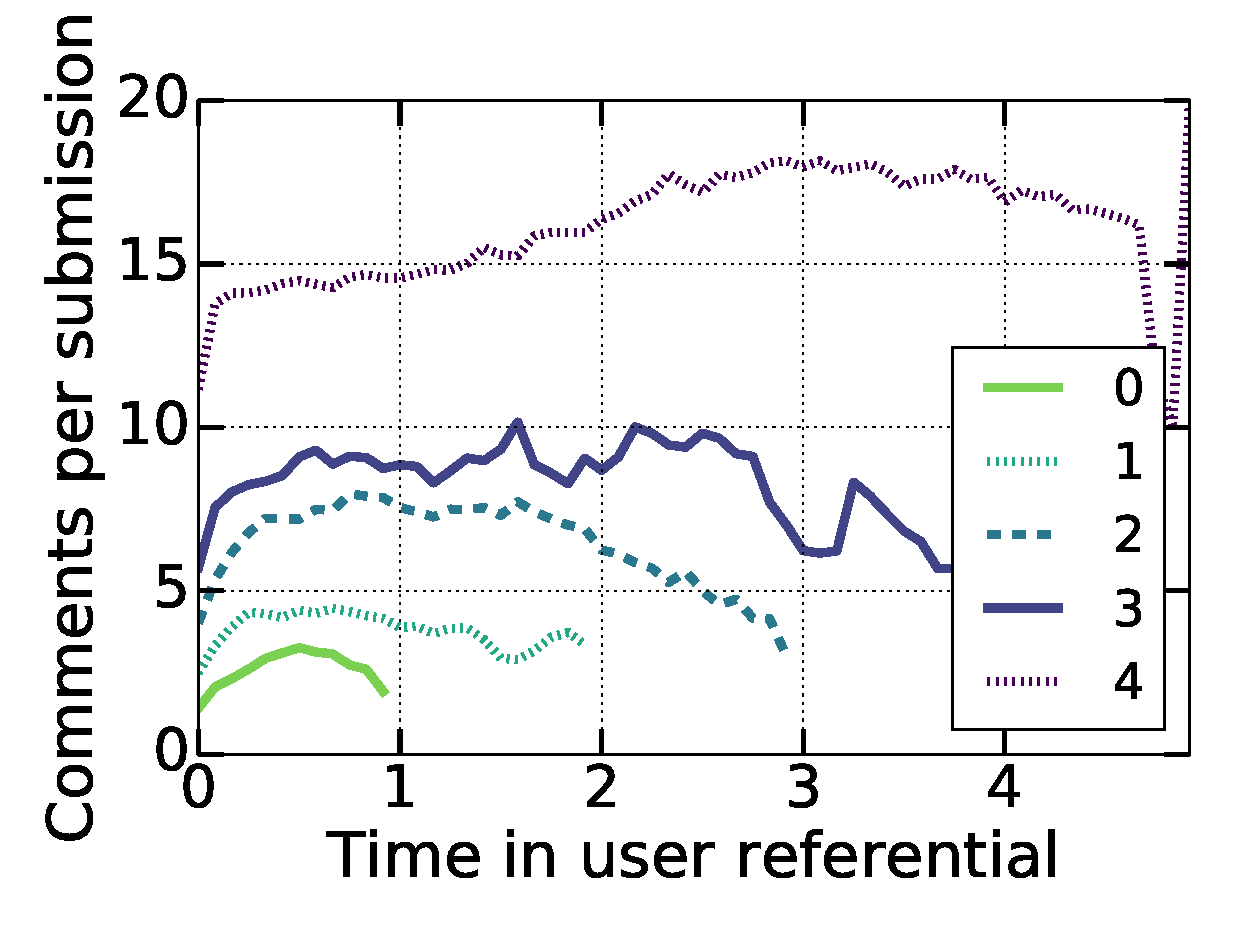
\includegraphics[scale=0.4]{./images/comments_per_submissions_for_surviving_year_for_2010.eps}
\caption{Caption}
\label{fig:comments_per_submissions_for_surviving_year_for_2010}
\end{figure}

\begin{figure}[!tb]
\centering
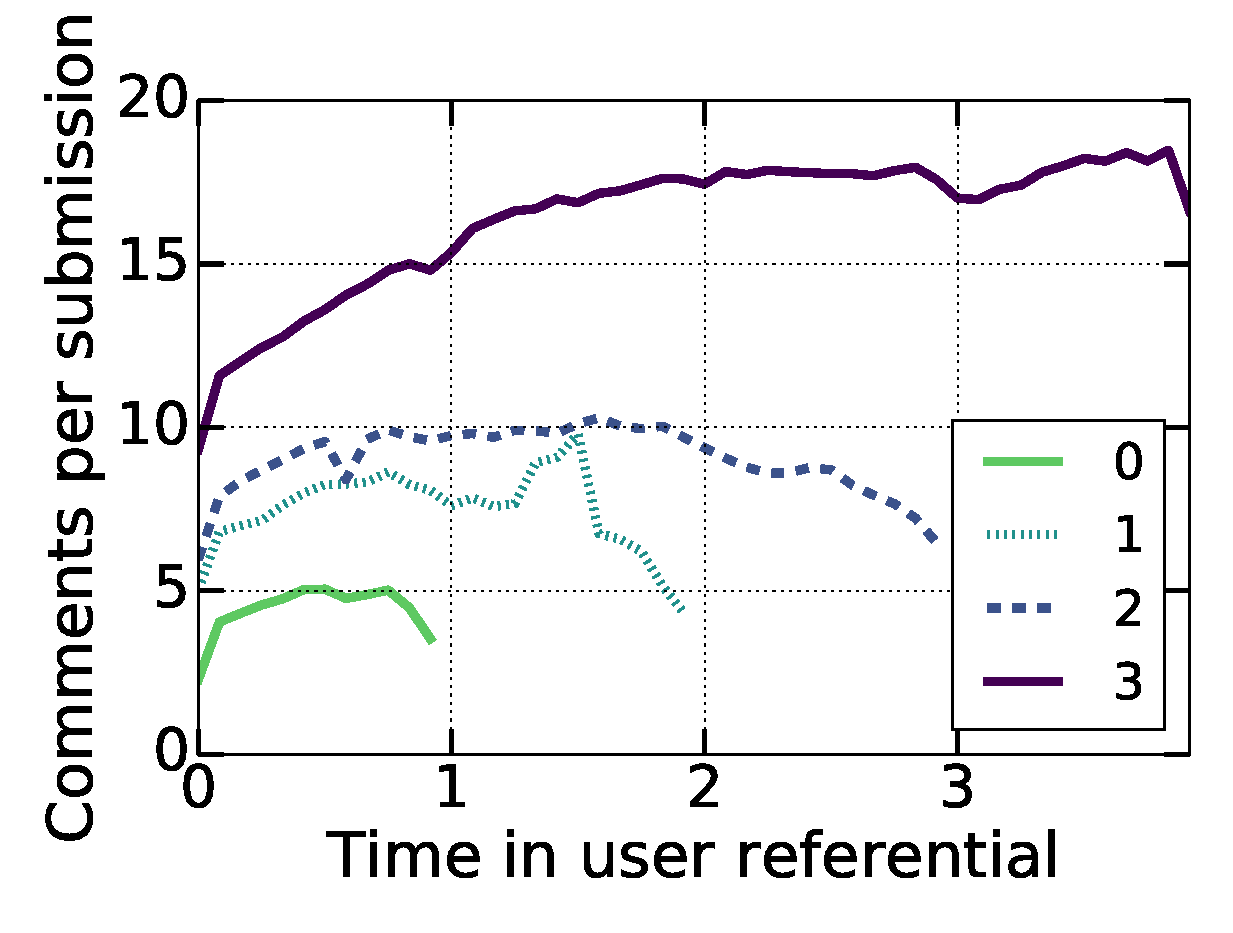
\includegraphics[scale=0.4]{./images/comments_per_submissions_for_surviving_year_for_2011.eps}
\caption{Caption}
\label{fig:comments_per_submissions_for_surviving_year_for_2011}
\end{figure}

\begin{figure}[!tb]
\centering
\includegraphics[scale=0.4]{./images/comments_per_submissions_for_surviving_year_for_2012.eps}
\caption{Caption}
\label{fig:comments_per_submissions_for_surviving_year_for_2012}
\end{figure}

\begin{figure}[!tb]
\centering
\includegraphics[scale=0.4]{./images/comments_per_submissions_for_surviving_year_for_2013.eps}
\caption{Caption}
\label{fig:comments_per_submissions_for_surviving_year_for_2013}
\end{figure}

\subsection{Users' Survival}

The simplest definition of an active user in reddit is to set a threshold date and define that every user that posted after that date is an active user and users that do not show any kind of behavior are ``dead''. This, however, is a limited interpretation of how users decide to stay or leave the network, specially if we want to analyse how this behavior changed over time. Also, since our users might always come back to the network at a later time, they might be ``reborn'', that means we have right censored data.

To account for these, we look at a one year window of time for each user. This way, we avoid the right censored data and the possibility that a user might have come back to the network at a later time. Given this, we segment users by their cohort and define that users active in the last 3 months of this one year window are active users. Based on this data manipulation, we present the Kaplan-Meier (cite) survival curve in Figure N.

\begin{figure}[!tb]
\centering
\includegraphics[scale=0.4]{./images/kaplan_meier_users.eps}
\caption{Kaplan-Meier estimator for one year of posting behavior for each user. Users for which the last posting day was in the first nine months of the one year window are considered ``dead''. This graph shows the percentage of surviving users per number of days since it first posted segmented by the cohort year the user joined the network.}
\label{fig:kaplan_meier_users}
\end{figure}

As previously mentioned, reddit shows a significant number of ``single time users'' that only post once in their existence. This can be seen in the initial drop in the first day. An interesting thing to see is that, although different cohorts level in different survival values, the ``user decay'' is similar throughout all of them. Not only that, but there is a general trend for older cohorts to die faster than younger ones. One possible explanation for that is that early reddit still lacked in content, with few subreddits to submit and few submissions to comment. This could lead to a higher number of users that did not stayed around after their initial impressions. 

\begin{figure}[!tb]
\centering
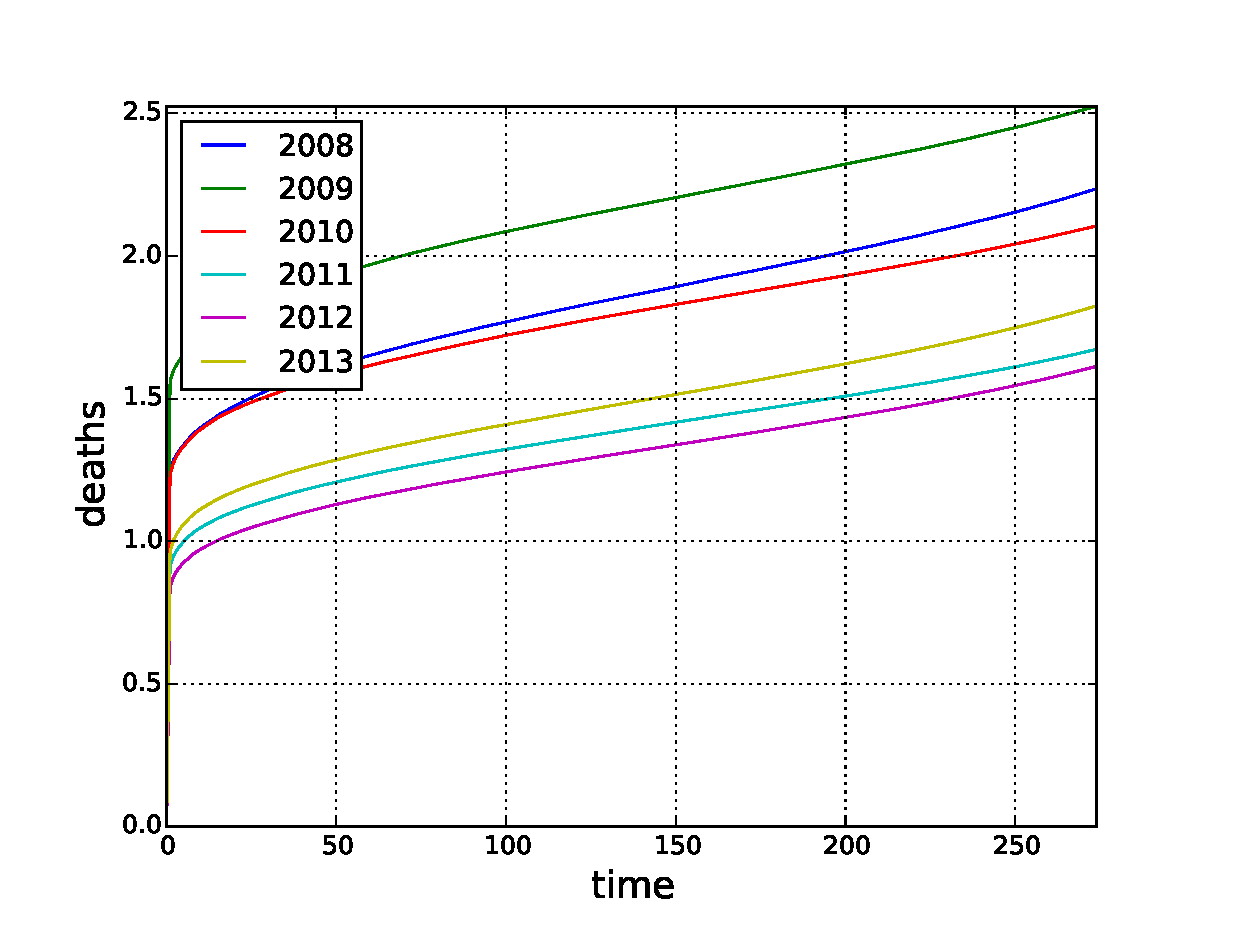
\includegraphics[scale=0.4]{./images/nelson_aalen_users.eps}
\caption{Caption}
\label{fig:nelson_aalen_users}
\end{figure}
